\chapter{ParaView Visualization}

The solver writes ParaView files in \texttt{output/}. The main file to open is:
\begin{center}
  \texttt{output/wave\_solution.pvd}
\end{center}
The scalar field to visualize is \texttt{u}. A useful representation is
\texttt{Surface With Edges}; to see the membrane as a moving surface one can
apply the \texttt{Warp By Scalar} filter to the same field.

The three-dimensional surface in ParaView is only a visualization. The
mathematical problem is still two-dimensional in space: the height represents
the scalar value \(u(x,y,t)\).

At the initial time the displacement is positive in the center of the square
and zero on the boundary. During the simulation the membrane oscillates: the
central displacement decreases, crosses zero, changes sign, and later returns
towards the initial shape. This is the behavior expected from the selected
manufactured solution, which has a cosine dependence in time.

\begin{figure}[H]
  \centering
  \begin{subfigure}{0.48\textwidth}
    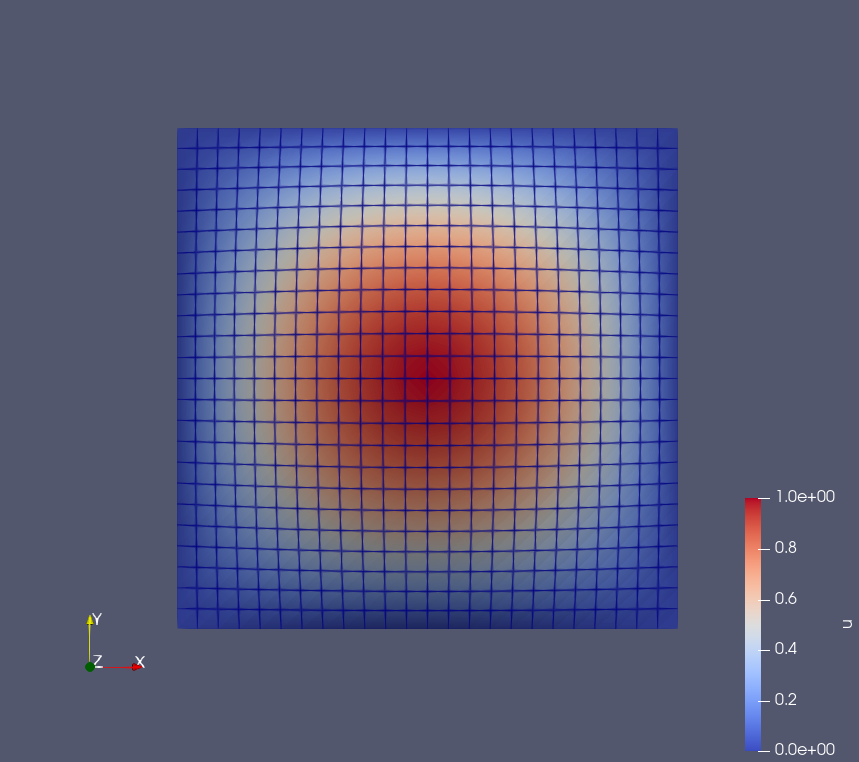
\includegraphics[width=\textwidth]{../../assets/paraview-screenshots/solution_u_t0_2d.png}
    \caption{Scalar field on the 2D mesh.}
  \end{subfigure}
  \hfill
  \begin{subfigure}{0.48\textwidth}
    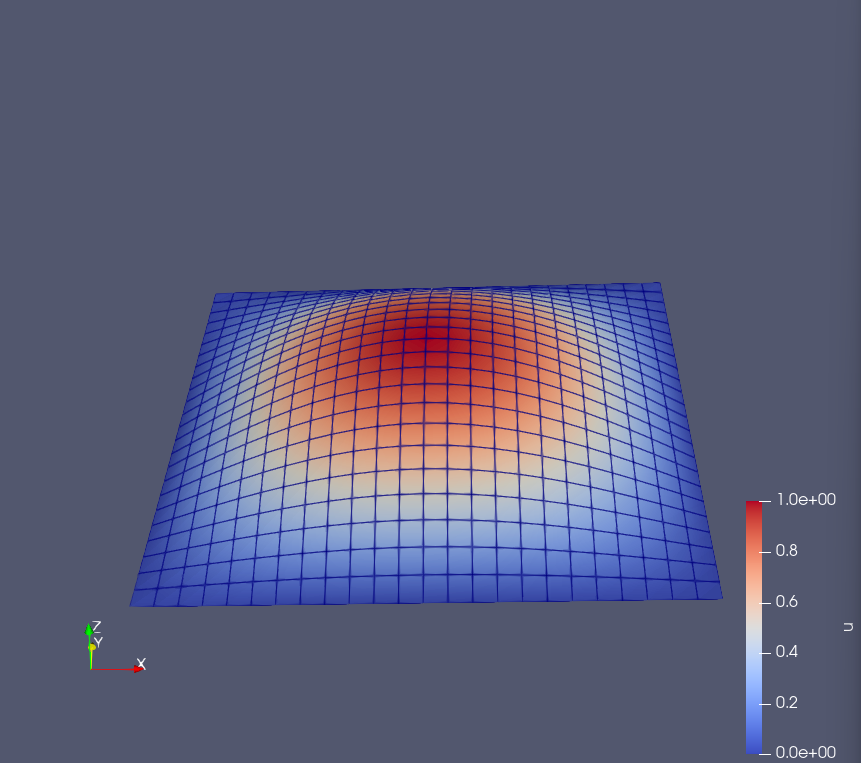
\includegraphics[width=\textwidth]{../../assets/paraview-screenshots/solution_u_t0_warped.png}
    \caption{Warped view of the same scalar field.}
  \end{subfigure}
  \caption{Initial displacement visualized in ParaView.}
\end{figure}

\begin{figure}[H]
  \centering
  \begin{subfigure}{0.48\textwidth}
    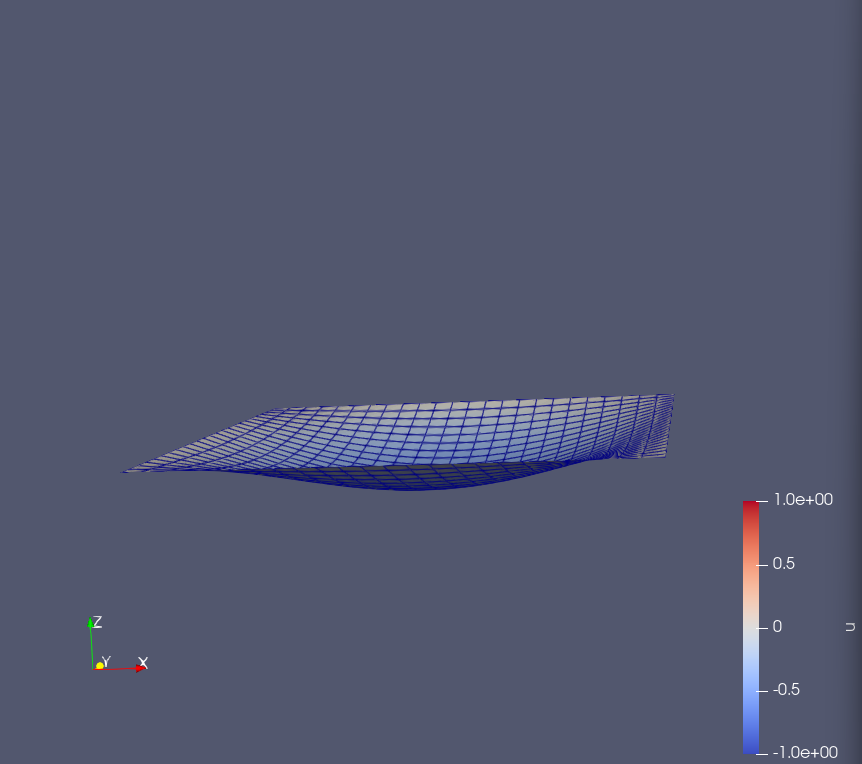
\includegraphics[width=\textwidth]{../../assets/paraview-screenshots/solution_u_t10_warped.png}
    \caption{Intermediate warped view.}
  \end{subfigure}
  \hfill
  \begin{subfigure}{0.48\textwidth}
    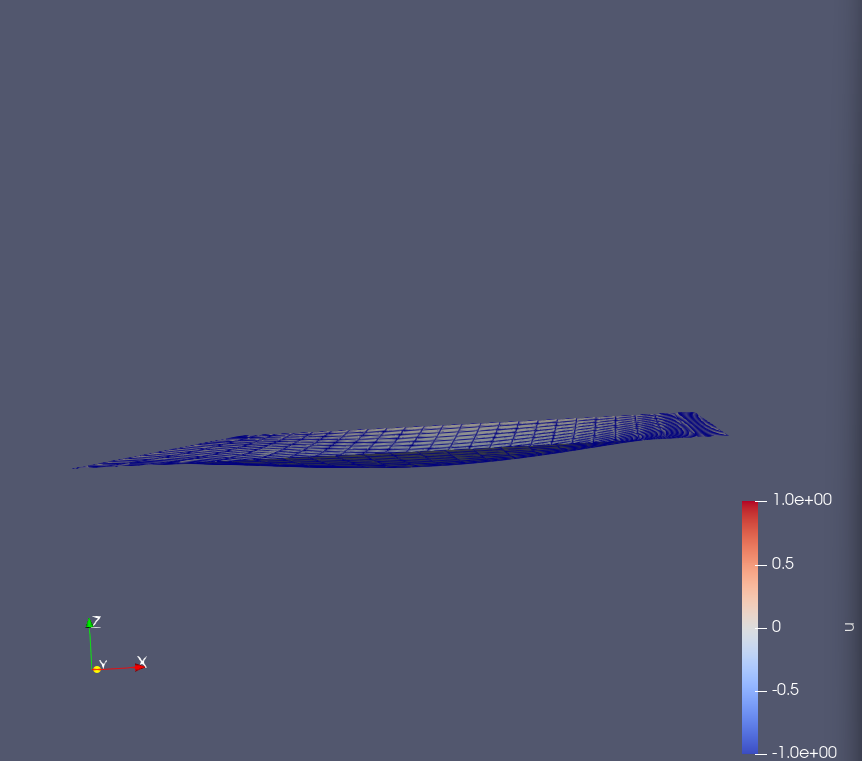
\includegraphics[width=\textwidth]{../../assets/paraview-screenshots/solution_u_t20_warped.png}
    \caption{Later warped view.}
  \end{subfigure}
  \caption{Time evolution of the membrane displacement in ParaView.}
\end{figure}

These are the group's existing qualitative screenshots. Their filenames
\texttt{t10} and \texttt{t20} do not establish physical times: no timestamp or
saved ParaView state accompanies them. They are retained as illustrations,
not used for error measurements or claimed to belong to the new convergence
study. For reproducible time labels, read the PVD time value in ParaView.
